\section*{Overview}

Heavy-light decomposition is the tree technique I use when a problem keeps asking for path queries or path updates
and the answer on one path can be merged from smaller contiguous pieces. The decomposition turns a tree path into a
small number of interval queries on a base array.

\section*{When to Use It}

Use it when:

\begin{itemize}
  \item queries are on paths between arbitrary vertices,
  \item each path answer can be combined associatively,
  \item point updates or interval updates inside a chain are manageable with a segment tree or Fenwick tree,
  \item simpler root-based tricks are not enough.
\end{itemize}

It is usually overkill for pure subtree queries, because Euler tour flattening alone often solves those.

\section*{Core Idea}

Pick one \textbf{heavy child} for each vertex: the child with the largest subtree. Follow heavy edges downward and
you get vertex-disjoint chains.

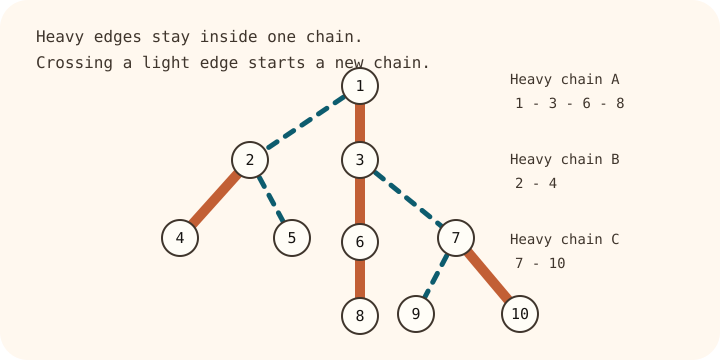
\includegraphics[width=\textwidth]{figures/chains.svg}

The important fact is not the picture itself but what it implies: every time a root-to-node walk crosses a light
edge, the remaining subtree size at least halves. So any root-to-node path crosses only \(O(\log n)\) light edges,
which means a path between two arbitrary vertices also breaks into only \(O(\log n)\) chains.

Once each vertex receives a position in the flattened chain order, every chain segment becomes an ordinary interval.

\section*{Operations}

The standard workflow is:

\begin{itemize}
  \item run one DFS to compute subtree sizes and identify the heavy child,
  \item run a second DFS to assign chain heads and flattened positions,
  \item store the flattened values in a segment tree,
  \item answer a path query by repeatedly climbing the deeper chain head.
\end{itemize}

If two vertices are on different chains, I query the deeper chain segment first, move to the parent of that chain
head, and repeat until both vertices land on the same chain.

\section*{Correctness Intuition}

Every tree edge belongs to exactly one chain step: either it is heavy and stays inside a chain, or it is light and
marks a jump between chains. Therefore the path between \(u\) and \(v\) can be partitioned into chain segments with
no overlap and no gaps.

Because each chain segment is stored contiguously in the flattened array, the segment tree answers each piece
correctly. Merging those piece answers in traversal order reconstructs the full path answer.

The logarithmic bound comes from light edges. Each time you move through a light edge toward the root, the current
subtree size at least doubles compared to where you came from, so there can be only \(O(\log n)\) such jumps.

\section*{Complexity Analysis}

\begin{itemize}
  \item preprocessing: \(O(n)\) for the two DFS passes,
  \item point update: \(O(\log n)\),
  \item path query: \(O(\log^2 n)\) with a segment tree,
  \item subtree query: \(O(\log n)\) if the note's flattened order is reused.
\end{itemize}

With more specialized data structures, the extra logarithm can sometimes be reduced, but \(O(\log^2 n)\) is the
contest default.

\section*{Implementation}

The reference implementation uses vertex values and supports:

\begin{itemize}
  \item build from an initial value per vertex,
  \item point assignment,
  \item path-sum query,
  \item subtree-sum query on the same flattening.
\end{itemize}

That version is enough for most introductory HLD problems. Edge-value problems usually store each edge's value on
the deeper endpoint and adjust the final interval boundaries accordingly.

\section*{Common Pitfalls}

\begin{itemize}
  \item Forgetting whether the structure stores values on vertices or on edges.
  \item Querying the final same-chain segment with the wrong inclusive range.
  \item Comparing vertex depth instead of chain-head depth when deciding which side to climb.
  \item Reusing the subtree interval trick without checking the flattening order still matches the decomposition DFS.
  \item Writing the segment tree correctly but assigning \texttt{head} or \texttt{pos} in the wrong order.
\end{itemize}

\section*{Practice Problems}

\begin{itemize}
  \item Path sum or path maximum queries with point updates.
  \item Queries that mix path operations and subtree operations in the same tree.
  \item Problems where HLD is the outer shell and the inner segment tree stores richer node states.
\end{itemize}

\section*{References}

\begin{itemize}
  \item \href{https://cp-algorithms.com/graph/hld.html}{cp-algorithms: Heavy-light decomposition}.
  \item \href{https://usaco.guide/CPH.pdf}{Competitive Programmer's Handbook}.
  \item \href{https://codeforces.com/catalog}{Codeforces Catalog}.
\end{itemize}
